\documentclass[10pt]{article}
\usepackage[polish]{babel}
\usepackage[utf8]{inputenc}
\usepackage[T1]{fontenc}
\usepackage{graphicx}
\usepackage[export]{adjustbox}
\graphicspath{ {./images/} }
\usepackage{amsmath}
\usepackage{amsfonts}
\usepackage{amssymb}
\usepackage[version=4]{mhchem}
\usepackage{stmaryrd}

\title{Zestaw 8 }

\author{}
\date{}


\begin{document}
\maketitle
\begin{center}
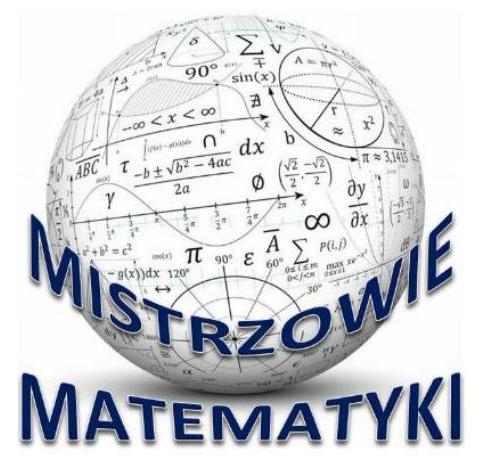
\includegraphics[max width=\textwidth]{2024_11_21_0d7cf2565ddbbb75f0d2g-1(1)}
\end{center}

\section*{GIMNAZJUM}
\begin{enumerate}
  \item Udowodnij, że jeżeli \(x^{2}+\frac{1}{x^{2}}\) jest liczbą całkowitą, to również \(x^{4}+\frac{1}{x^{4}}\) jest liczbą całkowitą.
  \item Dane są dwa okręgi, przecinające się w punktach \(A\) i \(B\). Przez punkt \(A\) poprowadzono sieczną obu okręgów, przecinającą pierwszy z nich w punktach \(A\) i \(K\), zaś drugi w punktach \(A\) i \(L\). Analogicznie przez punkt \(B\) poprowadzono sieczną przecinającą oba okręgi odpowiednio w punktach \(M\) i \(B\) oraz \(N\) i \(B\). Udowodnij, że odcinki \(K M\) i \(L N\) są równoległe.\\
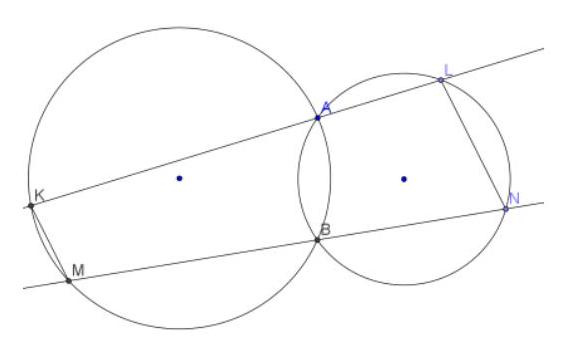
\includegraphics[max width=\textwidth, center]{2024_11_21_0d7cf2565ddbbb75f0d2g-1}
  \item Danych jest 111 dodatnich liczb całkowitych. Wykaż, że spośród nich można wybrać 11 takich liczb, których suma jest podzielna przez 11.
\end{enumerate}

\section*{LICEUM}
\begin{enumerate}
  \item Miara każdego kąta sześciokąta \(A B C D E F\) jest równa \(120^{\circ}\). Udowodnij, że symetralne odcinków \(A B\), \(C D\) i \(E F\) przecinają się w jednym punkcie.
  \item Uzasadnij, że dla dowolnego \(m\) całkowitego ułamek \(\frac{14 m+3}{21 m+4}\) jest nieskracalny.
  \item Wykaż, że obraz ortocentrum trójkąta w symetrii osiowej względem prostej zawierającej dowolny bok trójkąta należy do okręgu opisanego na tym trójkącie.
\end{enumerate}

Rozwiązania należy oddać do piątku 20 lutego do godziny 12.30 koordynatorowi konkursu panu Jarostawowi Szczepaniakowi lub swojemu nauczycielowi matematyki.

Na stronie internetowej szkoły w zakładce Konkursy i olimpiady można znaleźć wyniki dotychczasowych rund i rozwiązania zadań.


\end{document}